A tarefa de classificação de imagens consiste em predizer corretamente uma imagem como pertencente a uma classe previamente determinada. Um exemplo prático é a classificação da imagem de um \textit{oceano} como parte de uma classe denominada \textit{praia}. Uma forma de definir que certa imagem pertence à uma classe é especificar todas as regras que a caracterizam.
Porém, para a maioria dos casos isso é impossível. Considere imagens coloridas, com três canais de cores e de tamanho $256\times256$ pixels onde cada um desses 65536 pixels pode ser representado por $256^3$ combinações discretas de cores. Essa complexidade pode ser reduzida ao utilizar métodos de extração de características. Tais métodos visam representar uma imagem com um número significativamente menor de valores vetoriais. Utilizando-se tal representação, pode-se desenvolver métodos computacionais que consigam definir e identificar a qual classe pertence a imagem -- sem a necessidade de se codificar todas as regras possíveis -- por meio de algoritmos de Aprendizado de Máquina. Esses algoritmos possuem capacidade de generalização, crucial para classificar novos exemplos não contidos na base de imagens originalmente utilizada para o seu treinamento. Assim, ``aprendem'' a determinar a classe correta para as imagens de entrada. Em uma etapa posterior pode-se validar esse aprendizado, aplicando o algoritmo a novos exemplos não contidos no treinamento.

O reconhecimento de padrões em imagens possui aspectos particulares para cada aplicação. Apesar da grande variedade de extratores de características disponíveis, nem sempre é possível representar as imagens de maneira satisfatória. Isso porque existem conjuntos de características que dificultam a diferenciação entre as classes. Um dos objetivos da engenharia de atributos é encontrar quais são essas características que melhor discriminam as classes e, dessa forma, obter melhores resultados na etapa de reconhecimento. Para lidar com a deficiência da extração dessas características, é comum concentrar o maior esforço dessa tarefa no espaço de características já extraídas, utilizando transformações do espaço ou sistemas de classificação complexos. No entanto, imagens obtidas de diferentes fontes, como imagens naturais, de microscopia, telescopia e tomografia, possuem características que podem ser exploradas além dos métodos clássicos. Por isso é importante investigar métodos de processamento e preparação de imagens antes da etapa extração, ao invés de lidar com a má representação das imagens. O uso desses métodos pode revelar características latentes, não visíveis nas imagens originais. Tais características podem melhor descrever certas classes, pois melhoram o conjunto de representações de imagens fornecidas à etapa de classificação. Em dois estudos relacionados, é possível identificar a diferença da performance para problemas de classificação de imagens após o uso do pré-processamento. Em \citeonline{Rocha2010}, os autores atingem acurácia acima de 98\% na classificação de frutas após investigar alterações nos parâmetros de aquisição, realizar o pré-processamento e obter a segmentação. Já em \citeonline{Kanan2012}, os autores indicam que o método utilizado para obter a imagem em escala de cinza, pode impactar significativamente a classificação final de diversas bases de imagens.

Considerando que é comum realizar a extração de características a partir da imagem original, sem preocupação com a preparação da imagem, o enfoque desta pesquisa é na etapa de pré-processamento, destacada na Figura~\ref{fig:etapascanonicas}. Nela, ilustra-se as etapas canônicas do reconhecimento de padrões, desde a aquisição da imagem até sua posterior classificação. As etapas de pré-processamento e segmentação -- apresentadas em destaque no \textit{pipeline} -- são normalmente pouco exploradas, quando comparadas com as etapas posteriores.

\begin{figure}[!htbp]
 \begin{center}
   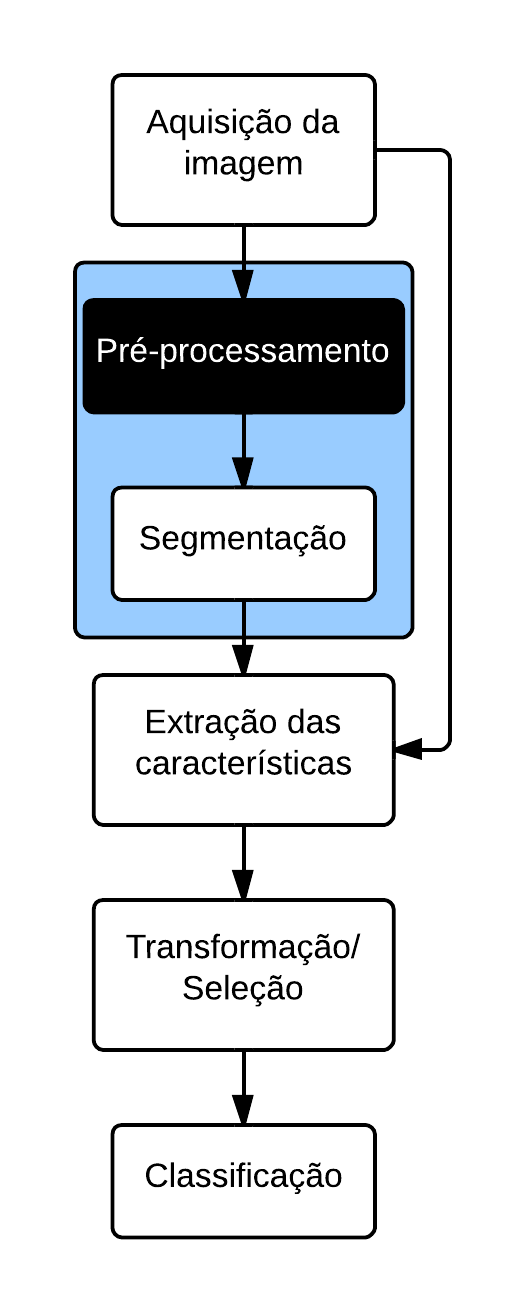
\includegraphics[width=0.3\linewidth]{figuras/flow.png}
 \end{center}
 \caption[Etapas canônicas do reconhecimento de padrões desde a aquisição da imagem até sua posterior classificação.]{Etapas canônicas do reconhecimento de padrões desde a aquisição da imagem até sua posterior classificação. As etapas de pré-processamento e segmentação -- apresentadas em destaque -- são normalmente pouco exploradas, quando comparadas com as etapas posteriores. O enfoque desse estudo é dar maior atenção à etapa de pré-processamento. \\ \textit{Fonte:~Elaborado pela autora.}}
 \label{fig:etapascanonicas}
\end{figure}

Primeiro, propõe-se a redução da complexidade do problema no início do processo do reconhecimento, ao quantizar as imagens antes da extração de características. Embora a quantização normalmente faça parte do \textit{pipeline}, faltam estudos que descrevam o método de quantização e seus parâmetros. Ao negligenciar essa etapa, perde-se a oportunidade de redução da dimensionalidade do vetor de características e/ou do tempo de execução das etapas posteriores.

O desbalanceamento de classes também se apresenta como um obstáculo para que a classificação de imagens seja satisfatória. Esse problema é caracterizado pela diferença entre o número de exemplos disponíveis para cada classe da base de imagens. Em bases médicas, por exemplo, a quantidade de imagens relacionadas com uma doença rara é menor do que as imagens de pacientes sem a doença. Nessas situações, em que as imagens representam eventos importantes porém menos frequentes, o sistema de classificação pode ter problemas para lidar com a classe minoritária. Normalmente esses sistemas dão preferência à predição da classe majoritária, prejudicando a classificação da minoritária.  Muitos métodos de transformação do espaço de características e de classificação assumem que as classes da base estão balanceadas, o que nem sempre é verdade.

Com o objetivo de promover o rebalanceamento de classes, algumas pesquisas sobre os efeitos da sobreamostragem em dados de aprendizado de máquina já foram realizadas~\cite{Kuncheva2004,Chawla2002}. O método mais divulgado na literatura é conhecido como \sigla{SMOTE}{\textit{Synthetic Minority Over-sampling Technique}}. Este método propõe a geração de exemplos artificiais a partir dos vetores de características originais das classes minoritárias. Por outro lado, não há registro conhecido de um estudo dessas técnicas em dados de informação \emph{visual} para o rebalanceamento de classes. A geração de imagens artificiais (ou sintéticas) é uma tarefa comum, mas não para o rebalanceamento de classes. Em \citeonline{Xie2016}, os autores utilizam um modelo generativo de uma CNN (\textit{Convolutional Neural Network}) para sintetizar imagens realistas. Essas imagens foram geradas, mas não utilizadas como entrada para um algoritmo de classificação ou no treinamento da própria rede. Propõe-se, portanto, a geração de imagens artificiais a partir do processamento das imagens originais, com o objetivo de rebalancear a base de imagens e consequentemente o modelo criado para a classificação. A fim de validar o método proposto, este é comparado com o SMOTE.

De maneira sumária, \textbf{esta pesquisa busca melhorar a classificação de imagens, com foco no rebalanceamento de classes e na quantização de imagens, ambos aplicados antes da extração de características.} Os resultados obtidos, posteriormente apresentados nos Capítulos \ref{cap:resultados-quantizacao} e \ref{cap:resultados-geracao}, demonstram o potencial do processamento de imagens antes da extração de características.

% Além disso, é fornecido uma visualização do espaço de características após o rebalanceamento das classes, crucial para analisar se as novas características extraídas são relevantes, ou seja, se adicionam informações que estavam latentes ao aprendizado. Os resultados também demonstram que a quantização das imagens permite obter vetores de características mais compactos e, ao mesmo tempo, com maior capacidade de discriminação entre classes.

% %--------------------------------------------------------------------------------
% \section{Contextualização}
%
% O grupo de pesquisa em Visualização, Imagens e Computação Gráfica (VICG), do Instituto de Ciências Matemáticas e de Computação (ICMC), tem atuado nas áreas de apoio para a classificação de coleções de imagens. Os trabalhos do grupo estão relacionados à visualização de informação com projeções multidimensionais e árvores~\cite{Joia2011}, assim como à extração de características e classificação de coleções de imagens~\cite{Paiva2011}. No que tange o processamento de imagens digitais, \citeonline{Picon2011} e \citeonline{Ponti2013} focam no pré-processamento para obter melhores resultados da classificação.
%
% Ainda, \citeonline{Paiva2011} mostraram que os espaços de características formados por cor e textura podem ser melhorados. Porém, há um limite até o qual as características podem ser transformadas, ou selecionadas, de forma a garantir a discriminação entre as classes. Tal projeto atua na investigação de métodos que permitam gerar espaços de características com maior discriminação entre as classes, facilitando assim a classificação.



%--------------------------------------------------------------------------------
\section{Hipóteses}

Conforme anteriormente mencionado, muitos aspectos influenciam a performance da classificação de coleções de imagens. É comum encontrar bases cuja extração de características é considerada difícil. Ou seja, nas quais algoritmos canônicos de extração não conseguem extrair características que diferenciem bem as classes, prejudicando sua posterior classificação. Nessa situação, normalmente tenta-se lidar com as particularidades das características extraídas através de transformações no espaço de atributos ou mesmo projetando classificadores mais elaborados. Acredita-se que, ao invés disso, é importante investigar métodos de processamento e preparação de imagens antes da extração das características.

A hipótese é que explorar etapas do processamento de imagens melhora a discriminação entre classes de uma coleção de imagens. Dois cenários são especificamente abordados:

\begin{itemize}

  \item \textbf{Utilizar um número reduzido de cores -- juntamente com um método de quantização apropriado, antes da extração de características -- pode permitir obter vetores de características mais compactos e com maior capacidade de discriminação entre classes.} Melhorando, assim, a classificação e diminuindo a complexidade do sistema. Além disso, analisa-se como diferentes métodos de quantização afetam ambas extração de características e posterior redução de dimensionalidade.

  \item \textbf{A geração de imagens artificiais como preparação para a extração de características pode melhorar a acurácia da classificação, quando comparada à geração de exemplos artificiais no espaço de atributos.} Ou seja, gerar novas imagens artificiais — que serão posteriormente reduzidas a atributos — pode apresentar melhores resultados para a classificação do que o \textit{bootstrap} de atributos artificiais.

\end{itemize}

\section{Contribuições}

\begin{description}
\item[Contribuição geral] \

Investigar os métodos de pré-processamento de imagens de forma a preparar uma coleção de imagens para a extração de características. Observa-se o efeito da quantização de imagens e do balanceamento do número de instâncias de diferentes classes na classificação.

\item[Contribuições específicas] \

  \begin{itemize}

    \item Demonstrar que é possível obter vetores de características compactos e efetivos ao extrair características de imagens com níveis reduzidos de intensidade a um custo computacional baixo. Reduzindo assim, o tamanho do vetor de características de métodos de descrição de cor após a quantização, e possibilitando a redução do tempo de processamento para os métodos de descrição de textura;

    \item Demonstrar que a geração de imagens artificiais utilizando métodos de processamento --- como borramento, mistura e combinação de imagens --- pode contribuir com o balanceamento entre classes (em se tratando de problemas de classes desbalanceadas). Melhorando, dessa forma, o \textit{f1-score} resultante de algoritmos de classificação, quando comparada à geração de exemplos artificiais no espaço de atributos (SMOTE) e à classificação da base original.

  \end{itemize}


\item[Contribuições em código e reproducibilidade] \

O código desenvolvido durante esta pesquisa, no que tange a geração artificial, está disponibilizado em \url{https://github.com/GabiThume/msc-src}. Já a implementação da quantização está disponível em \url{http://dx.doi.org/10.5281/zenodo.15932}. Esses repositórios correspondem à última versão do código para possível reprodução da pesquisa.

\end{description}

%--------------------------------------------------------------------------------
\section{Estrutura do documento}

Esta dissertação inicia apresentando os fundamentos necessários para a definição dos métodos utilizados nos experimentos. Esses métodos são então discutidos e, após, os resultados da quantização e da geração artificial são mostrados. O conteúdo está estruturado como segue.

\begin{description}
\item [Capítulo~\ref{cap:revisao}:] são conceituados os principais fundamentos necessários para o desenvolvimento desta pesquisa: pré-processamento de imagens, extração de características, desbalanceamento de classes, redução de dimensionalidade e a classificação de imagens.

\item [Capítulo~\ref{cap:quantization}:] a redução do número de intensidades de cor utilizando métodos de quantização antes da etapa de extração de características é descrita.

\item [Capítulo~\ref{cap:metodo}:] descreve-se os métodos de processamento utilizados para a geração artificial de imagens -- sobre as imagens originais -- com o objetivo de rebalancear classes.

\item [Capítulo~\ref{cap:resultados-quantizacao}:] os resultados obtidos com a quantização de imagens são apresentados e discutidos.

\item [Capítulo~\ref{cap:resultados-geracao}:] os experimentos com a geração de imagens artificiais para o rebalanceamento de classes são apresentados e seus resultados discutidos.

\item [Capítulo~\ref{cap:conclusoes}:] conclui as contribuições deste trabalho e apresenta os trabalhos futuros.

\end{description}
